% !TEX program = pdflatex
% !TEX root = main.tex

%----------------------------------------------------------------------------------------
\documentclass[a4paper,10pt]{article}

% Basic packages
\usepackage[utf8]{inputenc}
\usepackage{graphicx}
\usepackage{float}
\usepackage{amsmath}
\usepackage{amssymb}
\usepackage{amsthm}
\usepackage{multicol}
\usepackage{enumitem}
\usepackage{subcaption}
\usepackage{listings}
\usepackage{xcolor}
\usepackage{tikz}
\usepackage{changepage}

\usepackage{listings}
% \usepackage[T1]{fontenc}
% \usepackage[utf8]{inputenc}

\usetikzlibrary{positioning}
\usepackage[export]{adjustbox}
\usepackage[margin=2.5cm]{geometry}
\graphicspath{{images/}}
\usepackage{multirow}

% Load custom thesis style from config directory
\usepackage{config/thesis}

% Code listings
% \lstset{
%   basicstyle=\ttfamily\small,
%   frame=single,
%   columns=fullflexible
% }

% Thesis information
\thesistype{Specialisation Project (VT2)}
\thesistitle{Enhanced Platform for Investment Analysis}
\thesiscontext{Mixed-Integer Linear Programming Optimization Model for Integrated Energy Systems in Python}
\thesisdate{\today}
\thesissemester{HS2024}
\keywords{mixed-integer linear programming, MILP, quantitative modeling, python, strategic planning, optimization, asset valuation, power-flow, platform, forecasting, energy trading}

% Author information
\author{Rui Vieira}
\authorinstitute{Institute of Product Development and Production Technologies (IPP)}
\degree{Master of Science in Engineering}
\studyprogram{Business Engineering, MSc in Engineering}
\studyprogramlink{https://www.msengineering.ch/profiles/engineering-and-it/business-engineering}

% Supervisor information
\supervisorA{Dr. Andrea Giovanni Beccuti}
\supervisorAmail{giovanni.beccuti@zhaw.ch}
\supervisorAweb{https://www.zhaw.ch/en/about-us/person/becc}
\supervisorAinstitute{IEFE Model Based Process Optimisation}
\supervisorAinfo{%
    \supnameA\\
    \supinstituteA\\
    Email: \href{mailto:\supmailA}{\supmailA}\\
}

%----------------------------------------------------------------------------------------
\begin{document}

% Front
\begin{titlepage}

\begin{center}

\textup{\small {\bf Specialisation Project (VT) } \\  HS2024}\\[3.0in]

% Title
\fontsize{20}{24}\selectfont
\textbf {Platform for Investment Analysis}\\
\normalsize Optimization Framework for Energy Asset Management using Linear Programming in Python\\[3.0in]


       

% Submitted by
\normalsize Submitted by \\[0.2in]
\textbf{Rui Vieira}\\
Business Engineering Profile\\
IPP Institute of Product Development and Production Technologies\\

\vspace{.2in}




\vspace{.3in}

% Bottom of the page
\includegraphics[width=0.4 \textwidth]{images/mse.png}\\[0.1in]

January 2025

\end{center}

\end{titlepage}
% !TEX root = ../main.tex

%----------------------------------------------------------------------------------------
% IMPRINT
%----------------------------------------------------------------------------------------

\thispagestyle{empty}
\vspace*{\fill}

\noindent
{\bfseries  \Large Imprint}
\vspace{0.75cm}

\begin{footnotesize}

% Project information
\begin{flushleft} 
\begin{tabular}{ @{}lp{0.64\textwidth}@{} } 
    \emph{Project:}  & \ttype\\ 
    \emph{Title}:    & \ttitle\\
    \emph{Author}:   & \authorname\\
    \emph{Date}:     & \tdate\\
    \emph{Keywords}: & \keywordnames\\
\end{tabular}
\end{flushleft}

\vspace{0.75cm}

% University information
\noindent
\begin{minipage}[t]{0.95\textwidth}
\begin{flushleft} 
\emph{Study program:}\\
\href{\studyproglink}{\studyprog}\\
\href{\univlink}{\univname}
\end{flushleft}
\end{minipage}

\vspace{1.1cm}

\noindent
\begin{minipage}[t]{0.50\textwidth}
\begin{flushleft} 
\emph{Supervisor:}\\
\supinfoA
\end{flushleft}
\end{minipage}
\begin{minipage}[t]{0.45\textwidth}

    \begin{flushleft} 
\ifdefempty{\supnameB}
{}
{
    \emph{Supervisor 2:}\\
    \supinfoB
}
\end{flushleft}
\end{minipage}


\end{footnotesize}

\newpage

% Abstract
% !TEX root = ../main.tex

%----------------------------------------------------------------------------------------
% ABSTRACT PAGE
%----------------------------------------------------------------------------------------

\begin{abstract}
This work presents an integrated investment framework for energy systems, focusing on 
optimal technology selection and placement of electrical generation, conversion, and storage assets. The core 
engine combines DC Optimal Power Flow (DC-OPF) simulations with linear programming (using the PuLP solver) to 
evaluate both technical feasibility and economic viability across a multi-scenario analysis. A 9-bus test network 
provides the backdrop for a reduced ten distinct cases, each featuring a unique mix of conventional (nuclear, gas) and 
renewable (solar, wind) power plants, supplemented by battery storage of varying capacities.

To balance computational efficiency with seasonal realism, the annual horizon is divided into three representative 
weeks (summer, winter, and spring/autumn), whose costs and operations are subsequently scaled to form a full-year 
analysis. This approach reveals significant seasonal differences in storage utilization even enabling clean assets to
compensate for the cost of conventional generation.

\begin{figure}[H]
    \centering
    \includegraphics[width=0.6\textwidth]{images/soc_5.png}
    \caption{Summer/Winter battery SoC profile comparison -- Scenario 5}
    \label{fig:soc5}
\end{figure}

In scenarios featuring abundant solar generation, the SoC frequently reaches its upper limits, highlighting the 
potential for upsizing or more flexible operational strategies—such as battery leasing or modular additions—to 
capture peak renewable output.

An economic sensitivity analysis underscores the strong influence of high-cost resources during extreme load 
conditions, causing a disproportionate rise in total costs when reliance on expensive generation escalates. 
Meanwhile, scenarios with nuclear-dominated baseload exhibit lower operational cost volatility but may still 
benefit from targeted storage deployment to manage residual demand swings. AI-assisted reporting consolidates 
these findings by identifying cost drivers, optimal technology mixes, and operational bottlenecks across all 
scenarios. Notably, Scenario7’s balanced blend of nuclear, solar, and wind with moderate battery support emerges 
as the most cost-effective configuration, while Scenario4, featuring gas-fired generation and multiple storage 
units, proves the least favorable in terms of net present value (NPV).

Overall, the proposed framework bridges technical dispatch simulation and investment analysis, guiding stakeholders 
in designing resilient, economically viable energy systems. Future enhancements include broader maintenance modeling, 
real-time price integration for advanced arbitrage strategies, and further prompt-engineering improvements to refine 
AI-driven reporting and decision support.

\textbf{Keywords:} \keywordnames

%DC-OPF, Investment Analysis, Linear Programming, Renewable Integration, 
%Power Systems Planning, Asset Placement Optimization
\end{abstract}
\newpage

% Table of contents
\setcounter{tocdepth}{2}
\tableofcontents
\newpage

% Main content
\newpage
\section{Introduction}
\label{sec:intro_lit}

\subsection{Context and Motivation}
Electricity powers everything: homes, factories, and even the internet. 
Global energy demand is rising, and the shift to renewables like solar and wind is accelerating. But, 
this transition brings new challenges. Renewables are unpredictable, and increasing digitalization means 
more volatile and less controllable demand. Recent blackouts have exposed how dependent we are on the grid, 
and how easily disruptions cascade to other critical infrastructure, including the telecom network. 
This makes planning both short- and long- term demand or renewable generation more urgent than ever.

Building on last semester's linear programming (LP), we now introduce a mixed-integer linear programming (MILP) framework 
that optimizes both long-term investments and operations in an integrated way. In parallel, we developed a machine 
learning forecasting module to predict short-term (day-ahead) availability of renewable generation.

\subsection{Long-Term Planning with Mixed Integer Optimization}
The initial model, developed during the HS24 semester, addressed power flow and investment planning 
with a linear programming (LP) approach: fixed demand, hand-crafted scenarios, and only continuous 
variables for decision-making. While this enabled proof-of-concept studies, it had significant 
limitations and some lack of 'mathematical elegance'. The reliance on manually defined scenarios meant the true 
best investment strategy might never be evaluated. As a result, the model could not efficiently or systematically 
explore the full solution space for integrated planning.

The new version (VT2) adopts Mixed-Integer Linear Programming (MILP), where discrete (binary) variables 
enable us to model on/off states, asset retirements, maintenance cycles, and investment decisions in a unified, 
realistic manner~\cite{andersson2004power, wood2013power}. MILP co-optimizes capital and operational expenditure 
(CAPEX and OPEX), preventing suboptimal investment timing or dispatch caused by treating planning and operation 
separately. A commercial solver (IBM CPLEX) is now used and previous open-source solver (GLPK via PuLP) who 
is dramatically outperformed with large MILP problems and lack of parallelization.

\subsection{Short-Term Forecasting with Machine Learning}
Short-term forecasting of PV and wind is critical for grid operation. Methods range from simple persistence 
baselines to advanced ML models. We benchmarked several, ultimately using gradient boosting decision trees for primary 
forecasting and SARIMA as a baseline~\cite{grzebyk2021xgboost, zhong2020xgboost}. This enables to create a baseline 
model to predict electricity availability hence predict electricity spot prices based on single- imporant assets

Python’s mature ecosystem makes it the dominant platform for optimization and ML in energy systems. We leverage 
libraries such as scikit-learn, and statsmodels. Goal is to provide a baseline model to understand which factors drive
the electricity availability in the short-term.

%--------------------------------
% \section{Introduction}

% \subsection{Context \& Motivation}
% Electricity powers everything: homes, factories, even the servers running the latest 
% AI tools. The world's hunger for energy keeps rising, and the shift to renewables 
% like solar and wind is only speeding up. But that switch brings headaches: solar and 
% wind aren't predictable, and as more things go digital, unpredictable spikes can shake 
% the whole grid. Recent blackouts have made us realize how dependent we are on 
% the grid and often forget that internet is for now no existing without electricity.
% It's clear: we need to get better at planning for both the next hour and the next decade, 
% while also pushing for the integration of renewables sources of energy into the grid.

% \subsection{VT1 Bottlenecks}
% In the first version (VT1), we built a model that handled power flow and investment, 
% testing it on a handful of scenarios we set up by hand. The basics worked:
% \begin{itemize}
%     \item Demand was fixed and didn’t adapt.
%     \item Each scenario had to be loaded and managed manually.
%     \item The math (LP) let us solve problems, but skipped things like startup costs or 
%     on/off states for power plants.
%     \item We had to glue things together with custom scripts.
% \end{itemize}
% This setup proved the idea, but it missed the mark when it came to real-world details—
% especially picking the best grid setup based on cost and performance.

% \subsection{Goals and Scope of VT2}
% VT2 takes a major step forward, tackling the main gaps from the first version 
% with a more advanced and realistic approach:

% \begin{itemize}
%     \item \textbf{Realistic operational modeling:} Instead of only using 
%     continuous variables, VT2 upgrades to mixed-integer linear programming (MILP). 
%     This lets us explicitly represent unit commitment—so power plants can 
%     switch on or off, model asset retirements and simulate maintenance.
%     Once the logic implemented, we are a few code lines away of also introducing minimum up/down times, 
%     or start-up costs models but these were not implemented in this version.
%     \item \textbf{Data-driven renewable integration:} the new version now incorporates 
%     historical and reanalysis weather data to generate realistic wind and 
%     solar production forecasts. This means we’re not just simulating “average” 
%     days, but capturing the variability and uncertainty that challenge the grid.
%     making it possible to stress-test decisions against extreme events, 
%     seasonal lows, and sudden surges in demand.
%     \item \textbf{Modular, robust codebase:} The entire model has been 
%     refactored into a modular Python package using \texttt{Poetry}. Automated 
%     testing and continuous integration ensure that every change is checked for consistency and reliability. This not only speeds up development but makes it easier to extend—whether that’s adding new assets, market mechanisms, or scenario types.
% \end{itemize}

% With these improvements, VT2 shifts from a simple prototype to a more robust 
% planning and decision-support tool. It can now assess investment and operational 
% strategies under high renewable shares, tight operational constraints, and 
% uncertain future conditions—laying the groundwork for future features like 
% demand response and market-clearing simulation.
% --- Literature and Toolchain Review ---
\section{Literature and Toolchain Review}

\subsection{Mixed-Integer Programming in Power-System Planning}
Mixed-Integer Programming (MILP) is an improved version of Linear Programming (LP) 
that allows to solve problems with discrete variables for example whether a unit is on or off
(unit commitment). Such binary decisions can not be modelled with pure linear programming.
This allows to integrate investment (capital expenditure) and operational (dispatch, or operating cost)
decisions into one optimization framework. One can co-optimize the true least-cost solution 
that considers both capex and opex together. \cite{andersson2004power, wood2013power}.

Formulating generation expansion planning (GEP) as an MILP captures the binary nature of building 
decisions (build vs. not build) and can include operational details like unit commitment. Despite being possible to include operation 
details such as minimum on/off time, rampe rates, etc. in the model, it was not done in this project.
Not only is it more realistic but it also avoids suboptimal decisions that could arise from 
treating planning and operation separately.

\subsection{Short-term PV/Wind Forecasting Methods}
Short-term forecasting of photovoltaic (PV) or wind power is vital for grid operations. 
Approaches include:
\begin{itemize}
    \item \textbf{Persistence/Empirical}: Simple baselines, e.g., assuming tomorrow equals today.
    \item \textbf{Physical/NWP}: Use weather forecasts and physical models for power prediction.
    \item \textbf{Statistical}: ARIMA/SARIMA and ARIMAX models learn from historical data and 
    exogenous variables \cite{predictive_modeling_notes}. They are interpretable and 
    data-efficient but limited for nonlinearities.
    \item \textbf{Machine Learning}: Methods like neural networks, SVR, and especially gradient 
    boosting (e.g., XGBoost) capture complex patterns and often outperform statistical models 
    when sufficient data is available \cite{grzebyk2021xgboost, zhong2020xgboost, scikit-learn}. 
    Gradient boosting is noted for its accuracy and speed in PV/wind forecasting.
    \item \textbf{Hybrid/Ensemble}: Combine models (e.g., ARIMA+ANN) for improved robustness, 
    though added complexity may not always yield better results.
\end{itemize}
Given these findings, we used gradient boosting (XGBoost) for forecasting, with SARIMA as a 
baseline.

\subsection{Solver Landscape and Selection}
Solving large MILPs requires robust solvers. Commercial options (CPLEX, Gurobi, Xpress) are 
state-of-the-art, offering fast solve times and reliability \cite{mitchell2011pulp, forrest2018cbc}. 
Open-source solvers (CBC, GLPK, SCIP, HiGHS) are free but generally slower and less robust. 
Benchmarks show Gurobi and CPLEX are typically 12--100x faster than CBC, and commercial solvers 
solve more instances to optimality \cite{mittelmann2023benchmarks}.

For this project, CPLEX was chosen for the sake of understanding the solver and for having a 
academic license. Additionally, CPLEX offers a Python API (docplex), which made integration with 
our Python-based workflow straightforward

\subsection{Python Ecosystem for Optimisation and ML}
This interoperability and abundance of libraries is a major reason Python is so dominant in these 
fields today. Our literature review also confirmed that many recent research works in energy systems 
adopt Python for similar tasks, citing its balance of user-friendliness and powerful capabilities

Below is a list of the most relevant libraries for optimization and machine learning:

\begin{itemize}
    \item For optimization, libraries like PuLP and Pyomo allow flexible model formulation and 
    solver switching \cite{mitchell2011pulp}. We used the CPLEX Python API (docplex) for direct 
    integration. 
    \item For ML, scikit-learn and XGBoost provide powerful tools for data processing and 
    forecasting. Others librairies such as PyTorch, TensorFlow, and Keras are the reference ones 
    for deep learning and neural networks \cite{scikit-learn}. 
    \item Statsmodels was used for time-series (SARIMA) modeling as a baseline model.
\end{itemize}

\newpage

\newpage
\section{Problem Definition and Scope}
\label{sec:problem-definition}

This chapter formalises the real-world planning task that the optimisation model is 
meant to answer and translates it into a mathematical decision problem. 
Section~\ref{sec:planning-horizon} fixes the temporal and geographical domain of 
the study; Section~\ref{sec:decision-variables} introduces the decision variables and 
system constraints that emerge from those boundaries.

\subsection{Planning Horizon and System Boundaries}
\label{sec:planning-horizon}

\textbf{Temporal horizon} \quad The study covers a multi-year horizon of
\[
Y=\{1,\dots,Y_{\max}\},\qquad Y_{\max}\in[10,30]
\]
counted from a common base year $y=1$. Each year is represented operationally by three one-week seasons (winter, summer, spring / autumn) that together sum to 52 weeks via weighting factors
\[
w_{\text{winter}}=13,\;w_{\text{summer}}=13,\;w_{\text{spri autu}}=26.
\]

\textbf{Geographical scope} \quad The network model is a single high-voltage control area comprising:
\begin{itemize}
    \item $|B|$ transmission buses,
    \item $|L|$ AC lines modelled with DC susceptance,
    \item $|G|$ generators (thermal, wind, solar),
    \item $|S|$ storage units (battery or pumped hydro), and
    \item deterministic in-area electrical demand profiles.
\end{itemize}

Interconnection with neighbouring systems is neglected; cross-border trading is implicitly captured by fixed-price imports already embedded in the marginal costs of thermal units. Environmental constraints (emissions, RES quotas) are likewise outside the present scope; they can be added later as linear constraints if needed.

\textbf{Uncertainty handling} \quad All time-series---load, wind and solar availability---are treated as perfect forecasts for the representative weeks. Inter-annual load growth is exogenous and applied through deterministic scaling factors $\gamma_y$. No stochasticity or scenario tree is modelled in Chapter~4; the MILP therefore produces a single, deterministic expansion path.

\subsection{Decision Variables and Constraints}
\label{sec:decision-variables}

The model couples long-term investment choices with short-term operation. Four families of variables are sufficient; all constraints remain linear.

\begin{center}
\begin{tabular}{llll}
Symbol & Nature & Description & Index sets \\
\hline
\textsf{build}\(_{a,y}\) & binary & 1 $\Rightarrow$ asset $a$ is commissioned in year $y$ & $a \in G \cup S,\;y \in Y$ \\
\textsf{inst}\(_{a,y}\) & binary (derived) & 1 $\Rightarrow$ asset $a$ is operational in year $y$ & same \\
u\(_{g,\sigma,y,t}\) & binary & Unit-commitment status of thermal generator $g$ & thermal $g$, $\sigma \in \Sigma, y, t$ \\
p\(_{g,\sigma,y,t}\) & continuous $\geq 0$ & Dispatch of generator $g$ (MW) & all $g,\sigma,y,t$ \\
c\(_{s,\sigma,y,t}\) & continuous $\geq 0$ & Storage charge (MW) & all $s,\sigma,y,t$ \\
d\(_{s,\sigma,y,t}\) & continuous $\geq 0$ & Storage discharge (MW) & all $s,\sigma,y,t$ \\
\textsf{soc}\(_{s,\sigma,y,t}\) & continuous $\geq 0$ & State of charge (MWh) & all $s,\sigma,y,t$ \\
f\(_{l,\sigma,y,t}\) & continuous & DC power flow on line $l$ (MW) & all $l,\sigma,y,t$ \\
\end{tabular}
\end{center}

(The current code base allows the UC binaries to be de-activated, but the formulation keeps the slot for future work.)

\subsubsection{Investment logic}
\begin{enumerate}
    \item \textbf{Chunk-based lifetime rule}
    \[
    \sum_{y'=y-L_a+1}^{y}\textsf{build}_{a,y'}\le 1
    \quad\forall a,\;y
    \]
    forbids commissioning the same asset twice within its lifetime $L_a$.
    \item \textbf{Installed-status definition}
    \[
    \textsf{inst}_{a,y}= \sum_{y'=y-L_a+1}^{y}\textsf{build}_{a,y'}
    \quad\forall a,\;y
    \]
    makes $\textsf{inst}$ a derived binary that switches on exactly in the years covered by the latest build.
    \item \textbf{Annualised CAPEX} – each installed asset incurs a fixed annuity $A_a$ (Section~4.2b) in every active year and zero otherwise.
\end{enumerate}

\subsubsection{Operational constraints}
\begin{enumerate}
    \item \textbf{Generator capacity}
    \[
    0\le p_{g,\sigma,y,t}\le P^{\max}_g
    \begin{cases}
    \alpha_{g,\sigma,t}\textsf{inst}_{g,y}, & g\in\{\text{wind},\text{solar}\}\\
    \textsf{inst}_{g,y}, & \text{thermal}
    \end{cases}
    \]
    where $\alpha$ is the time-varying availability profile.
    \item \textbf{Unit-commitment (optional)}
    
    If UC binaries are enabled:
    \[
    p_{g,\sigma,y,t}\le P^{\max}_g u_{g,\sigma,y,t}.
    \]
    \item \textbf{Storage dynamics}
    \[
    \text{soc}_{s,\sigma,y,t+1}=
    \text{soc}_{s,\sigma,y,t}+\eta^{\text{in}}_s c_{s,\sigma,y,t}
    -\frac{1}{\eta^{\text{out}}_s}d_{s,\sigma,y,t}
    \]
    with
    \[
    0\le\text{soc}_{s,\sigma,y,t}\le E^{\max}_s\textsf{inst}_{s,y}\quad\text{and}\quad
    \text{soc}_{s,\sigma,y,1}=0.
    \]
    \item \textbf{Nodal balance (Kirchhoff)}
    \[
    \sum_{g\in G_b} p_{g,\sigma,y,t}
    +\sum_{s\in S_b} (d_{s,\sigma,y,t}-c_{s,\sigma,y,t})
    +\sum_{l\in L^{\text{in}}_b} f_{l,\sigma,y,t}
    = \gamma_y \lambda_{b,\sigma,t}
    +\sum_{l\in L^{\text{out}}_b} f_{l,\sigma,y,t}
    \]
    \item \textbf{DC line limits}
    \[
    |f_{l,\sigma,y,t}|\le F^{\max}_l.
    \]
    \item \textbf{Season weighting}
    
    Operational cost is summed over $w_\sigma$ replicated weeks:
    \[
    \sum_{\sigma} w_\sigma\sum_t (\cdot).
    \]
\end{enumerate}

With these variables and constraints the model simultaneously decides what to build, when to build it and how to operate the system hour-by-hour in the representative weeks—while rigorously respecting lifetime, network and storage physics.

\subsection{Forecast Horizon and Accuracy Targets}
\label{sec:forecast-horizon}

The integrated workflow (see Figure~4-1) requires two nested time-axes:

\begin{center}
\begin{tabular}{llll}
Layer & Resolution & Span & Consumer \\
\hline
Forecast module & 1~h & $HF = 0\ldots48$~h rolling & feeds hourly PV/Wind expectations to the MILP \\
Optimisation core & 1~h (in-model) $\rightarrow$ 168~h representative weeks & $HO = 168$~h per scenario & determines UC, storage dispatch, capex \\
\end{tabular}
\end{center}

We therefore define a 48-hour look-ahead as the operational forecast horizon:
\begin{itemize}
    \item \textbf{0--6~h ahead (intra-day):} covers balancing-market bids and real-time redispatch.
    \item \textbf{6--24~h ahead (day-ahead):} coincides with spot-market gate closure.
    \item \textbf{24--48~h ahead (two-day stability buffer):} protects against low-pressure fronts and forecast drift that would otherwise trigger excessive start-ups in the MILP.
\end{itemize}

Accuracy targets are expressed in mean-absolute-error (MAE) on the hold-out calendar year 2024:

\begin{center}
\begin{tabular}{lll}
Horizon & Target MAE & Rationale \\
\hline
1~h & $\leq 5\%$ of mean load & real-time control margin \\
24~h & $\leq 8\%$ & day-ahead bidding error used by TSOs [ENTSO-E benchmark] \\
48~h & $\leq 10\%$ & keeps MILP recourse cost $<2\%$ of total cost (Section~6.2) \\
\end{tabular}
\end{center}

These thresholds guide model selection in Stages~0--4: any candidate whose cross-validated MAE breaches a band is discarded or re-tuned. Stage-3's Trim~+~BSFS~GBT currently meets the 1~h and 24~h targets and is within 0.6~pp of the 48~h goal; further feature pruning and ensembling are planned.

A horizon-decay analysis (to be added in Section~6.1) will chart MAE versus lead-time to ensure monotonic degradation and reveal any regime-specific bias (e.g., sunset spikes).

\subsection{Key Performance Indicators (KPIs)}
\label{sec:kpis}

To link forecasting quality with economic impact we track three KPI families:

\begin{center}
\begin{tabular}{llll}
Class & Symbol / Unit & Measurement Window & Purpose \\
\hline
Economic & $TC$ [€] -- total system cost (objective value) & per optimisation run & Primary goal: minimise net-present cost of generation, storage and purchases. \\
Computational & $T_{\text{solve}}$ [s] -- MILP wall-clock solve time \\ $\text{gap}_{\text{final}}$ [\%] -- optimality gap & per scenario \& sensitivity sweep & Confirms MILP tractability; target $T_{\text{solve}} \leq 600$~s and $\text{gap} \leq 0.1\%$ on baseline hardware. \\
Forecasting & MAE, RMSE [kWh] & rolling 48~h forecasts on 2024 hold-out & Inputs for stochastic/error-band scenarios; MAE is ranking metric, RMSE punishes spikes. \\
\end{tabular}
\end{center}

\textbf{How they interact}
\begin{enumerate}
    \item \textbf{Forecast $\rightarrow$ Economics:} Higher MAE inflates $TC$ via reserve and start-up penalties. Sensitivity runs will quantify the €/MAE gradient.
    \item \textbf{Forecast $\rightarrow$ Computation:} Poor forecasts enlarge the feasible region (more binaries switch), often raising $T_{\text{solve}}$.
    \item \textbf{Solver performance:} If $T_{\text{solve}}$ exceeds the rolling forecast refresh (1~h), operational viability is lost; hence the 600~s threshold.
\end{enumerate}

All KPIs will be logged per experiment run (MLflow for MAE/RMSE; CPLEX-log parser for $T_{\text{solve}}$) and summarised in Section~6. Metrics are reported with 95\% bootstrap CIs to reflect temporal autocorrelation.

\newpage

\newpage
\section{Linear to Mixed-Integer Programming Transition}
\label{sec:MILP_transition}
Building on last semester's investment model work~\cite{vierui2024vt1}, we now let the
model decide when to build or replace each asset.  To simply put it, we add binary variables 
to capture theassets availability and usage and define a new objective function 
balancing both investment and operational costs.

The previous linear (LP) formulation fixed the asset list ex-ante; any capacity
study meant running dozens of “what-if” scenarios offline.  In the MILP,
those scenarios collapse into one optimisation that jointly chooses
dispatch \emph{and} build schedule for the lowest net present cost. Running this logic over
multiple years, generates the possibility to assess when in a horizon, should an asset be built 
given its lifetime and associated cost.

\subsection{Key modelling ideas}
\label{ssec:MILP_methodology}

\begin{enumerate}[label=\textbf{\roman*}.]
  \item \textbf{Two binary variables per asset and year}\footnote{Upper-case sets:
        $\mathcal{A}$ assets, $\mathcal{Y}$ years, $\mathcal{B}$ buses.
        Lower-case indices: $a,\,y,\,b$ etc.}
        \begin{align*}
            z^{\text{build}}_{a,y} &= 
              \begin{cases}
                1 &\text{if asset $a$ is \emph{commissioned} in year $y$}\\
                0 &\text{otherwise}
              \end{cases},
            &
            z^{\text{on}}_{a,y} &= 
              \begin{cases}
                1 &\text{if asset $a$ is \emph{operational} in year $y$}\\
                0 &\text{otherwise.}
              \end{cases}
        \end{align*}

        Two binaries per asset per year are present in the model, but:
        \begin{itemize}
            \item Only the $z^{\text{build}}$ variables are truly “free” (decision variables).
            \item The $z^{\text{on}}$ variables are “dependent” binaries: each year’s installed status is determined (by constraint) as the sum of all unexpired builds.
        \end{itemize}

  \item \textbf{Lifetime-aware coupling}\\
        Each asset lives $L_a$ (lifetime) years.
        \begin{equation}
            \setlength{\arraycolsep}{2em}
            \begin{array}{rlrl}
                z^{\text{on}}_{a,y} = \displaystyle \sum_{\substack{y' \le y \\ y - y' < L_a}} z^{\text{build}}_{a,y'} 
                & \displaystyle \sum_{\substack{y' \le y \\ y - y' < L_a}} z^{\text{build}}_{a,y'} \le 1
            \end{array}
            \tag{2a, 2b}
            \label{eq:lifetime_link}
        \end{equation}
        \addtocounter{equation}{1}  % skips the unused (1) makes the next auto one (2)
        \noindent
        \begin{itemize}
            \item (a) says an asset is “on” if it was built in the last $L_a$ years
            \item (b) forbids more than one build : "at-most-one-build-per-lifetime"
            \item $y'$ is the year of the last build
        \end{itemize}

  \item \textbf{Capacity gating}\\
       Dispatch variables (Generator : $P^{\mathrm{gen}}$, storage power : $(P^{\mathrm{ch}},
       \text{and} P^{\mathrm{dis}})$ and state of charge : $E$) are multiplied by the installation flag $i_{a,y}$ .
       If an asset is not built, its capacity is mathematically zero.
       \[ 0 \leq X^{\text{asset}}_{a,y} \leq X^{\text{max}}_{a} \cdot z^{\text{on}}_{a,y} \]


  \item \textbf{Annualised CAPEX via Capital Recovery Factor (CRF)}\\
      Capital expenditure (CAPEX) is annualized using the Capital Recovery Factor (CRF).  It is an asset-specific financial metric used to calculate the annualized cost of an investment over its lifetime.
      The goal is to make investment and operational costs comparable in a single linear objective. It is defined as:
      \begin{equation}
      \text{CRF}_a \;=\; \frac{i\;(1+i)^{L_a}}{(1+i)^{L_a}-1},
      \qquad
      A_a \;=\; \text{CRF}_a \, \cdot\, C_a.
      \end{equation}
      \begin{itemize}
            \item $A_a$ is the \emph{annual} cost of owning one unit of asset $a$.
            \item $C_a$ is the \emph{capital cost} of asset $a$.
            \item $i$ is the \emph{interest rate} (depreciation rate between 5--10\%) 
      \end{itemize}
      
      The annulized cost brings a strong advantage in the context of a multi-year analysis.
      Instead of charging the full investment (CAPEX) upfront or at the end of an asset's lifetime, 
      the total cost is distributed evenly across each year that the asset is operational within the 
      optimization horizon.
      This approach has several technical and economic advantages:

      \begin{itemize}
            \item Each asset pays a fixed annual cost while installed, simplifying the objective.
            \item Only pay for years the asset is in use, avoiding end-of-horizon "distortions".
            \item Removes cost jumps at build/retire dates.
            \item The annuity is linear and easy to implement, unlike full discounted cash-flow tracking.
            \item Slight approximation error from annualizing if the asset is not used for all its lifetime, 
            but negligible in practice.
      \end{itemize}

      This is implemented in code as follows:
      \begin{lstlisting}[language=Python, numbers=none]
      def compute_crf(lifetime, discount_rate):
            # Capital Recovery Factor (CRF)
            if lifetime is None or lifetime <= 0:
                  return 1.0
            i, n = discount_rate, lifetime
            return (i * (1 + i)**n) / ((1 + i)**n - 1)
      
      # Annualized cost (annuity)
      annual_asset_cost = npv * compute_crf(lifetime, discount_rate)
      \end{lstlisting}

      In the optimization: The annualized cost is added for every year the asset is installed, for both 
      generators and storage units:
      \begin{lstlisting}[language=Python, caption=Objective function cost term]
      for y in years:
      total_cost += annual_asset_cost * gen_installed[(g, y)]
      \end{lstlisting}
      
      This modeling choice is implemented in \texttt{dcopf()} and post-processed in the cost analysis script. It ensures that costs are spread proportionally and that the cost function remains robust, regardless of asset timing or lifetime relative to the analysis horizon.

  \item \textbf{Load growth factor}\\
        To mimic a time-varying load through the years, the loads are scaled within the nodal-balance by a defined 
        factor $\gamma_y$. This induces a growing demand in the model without increasing the generation. 
        This induces a diversification of the generation mix through the years.
        \[
        \tilde D_{y} = \gamma_y\,D_{y}.
        \]
        It was decided to model the load growth factor as a global factor for all buses, but it could be extended to a 
        bus-specific factor.
\end{enumerate}

\newpage
\subsection{MILP formulation}
\label{ssec:MILP_implementation}

Only the constraints that changed vs.\ the LP are listed. For readability, the indices set such as $s$ (season) and $t$ 
(hour) were are omitted since per season or per hour concept are implied. Other non-relevant indices may be missing too.

\paragraph{A.~Investment constraints}
\begin{itemize}
  \item Lifetime link \eqref{eq:lifetime_link} (see above).
      \item Generator, storage power and energy limits as mentionned in the
        capacity gating bullet:
        \begin{itemize}
        \item Generator Output Limits:\\
            \begin{equation}
                  0 \leq P^{\text{gen}}_{a,y} 
                  \leq P^{\text{max}}_{a} \cdot z^{\text{on}}_{a,y}
            \end{equation}
    
        \item Storage Power Limits:\\
            \begin{equation}
                  \begin{aligned}
                        0 &\leq P^{\text{ch}}_{a,y} \leq P^{\text{max}}_{a} \cdot z^{\text{on}}_{a,y} \\
                        0 &\leq P^{\text{dis}}_{a,y} \leq P^{\text{max}}_{a} \cdot z^{\text{on}}_{a,y}
                  \end{aligned}
            \end{equation}
    
        \item Energy Capacity Limit:\\
            \begin{equation}
                  - E^{\text{max}}_{a} \cdot z^{\text{on}}_{a,y} \leq E_{a,y} \leq E^{\text{max}}_{a} \cdot z^{\text{on}}_{a,y}
            \end{equation}
      \end{itemize}
\end{itemize}

\paragraph{B.~Operational constraints (modified)}
\begin{itemize}

      
      \item Nodal balance with load scaling\\
            For each bus $b$, season $s$, year $y$, hour $t$:
            \begin{equation}
                  \sum_{a \in \mathcal{A}_b} P^{\text{gen}}_{a,y} +
                  \sum_{a \in \mathcal{A}_b} (P^{\text{dis}}_{a,y} - P^{\text{ch}}_{a,y}) +
                  \sum_{\ell \in \text{in}(b)} F_{\ell,y}
                  = 
                  \gamma_y \cdot D_{b} +
                  \sum_{\ell \in \text{out}(b)} F_{\ell,y}
                  \label{eq:nodal_new}
            \end{equation}
      
      The only change is the growth factor $\gamma_y$ on the demand term.
\end{itemize}

\paragraph{C.~Objective function}
\begin{equation}
      \min \quad
      \underbrace{\sum_{s \in \Sigma} W_s \sum_{y}\Bigl(\sum_{a} c_a \cdot P^{\text{gen}}_{a}\cdot z^{\text{on}}_{a}\Bigr )}_{\substack{\text{operating costs} \\ \text{OPEX}}}
      +
      \underbrace{\sum_{y}\Bigl(
      \sum_{a\in\mathcal{A}}
          A_a \;\cdot z^{\text{on}}_{a}\Bigr)}_{\substack{\text{investment costs} \\ \text{CAPEX}}}
  \end{equation}
  With:
  \begin{itemize}
      \item $W_s$: Number of calendar weeks represented by each season $s$ (e.g., winter = 13)
      \item Annualised CapEx per asset $a$ : $A_a = \mathrm{CRF}_a \cdot C_a$ 
  \end{itemize}  
Hence the MILP simultaneously finds the least-cost \emph{dispatch} and the cheapest \emph{build / replace} schedule over the planning horizon. It eliminates the need for external spreadsheets computing NPV and manual scenarios comparison.

\subsection{Implementation pipeline}
Figures \ref{fig:milp_internal_flow} and~\ref{fig:scripts_block}
show how CSV inputs and time-series flow through the four main Python
modules (\texttt{pre.py}, \texttt{network.py}, \texttt{optimization.py},
\texttt{post.py}) and finally into \texttt{cost.py} for the cost analysis. The code matches the
math 1:1.

%----------------------------------------------------------
\subsection{Investment analysis pipeline}
\label{ssec:milp_impl}
%----------------------------------------------------------

\subsubsection*{A.\ Overview and roles}

\begin{figure}[h!]
      \centering
      \begin{adjustbox}{width=0.8\textwidth}
      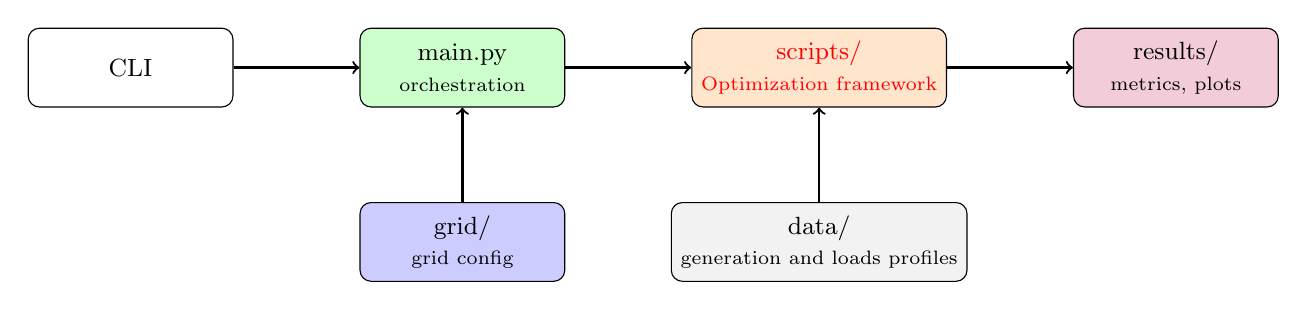
\begin{tikzpicture}[
          node distance=1.2cm and 1.6cm,
          every node/.style={font=\small, rounded corners},
          phase/.style={draw, fill=white!40, minimum height=1cm, minimum width=2.6cm, align=center},
          io/.style={draw, fill=blue!20, minimum height=1cm, minimum width=2.6cm, align=center},
          main/.style={draw, fill=green!20, minimum height=1cm, minimum width=2.6cm, align=center},
          opti/.style={draw, fill=orange!20, minimum height=1cm, minimum width=2.6cm, align=center},
          output/.style={draw, fill=purple!20, minimum height=1cm, minimum width=2.6cm, align=center},
          data/.style={draw, fill=gray!10, minimum height=1cm, minimum width=2.6cm, align=center},
          arrow/.style={->, thick}
      ]
  
      % Nodes
      \node[phase] (cli) {CLI};
      \node[main, right=of cli] (main) {main.py\\\scriptsize orchestration};
      \node[io, below=1.2cm of main] (grid) {grid/\\\scriptsize grid config};
      \node[opti, right=of main, text=red] (opti) {scripts/\\\scriptsize Optimization framework};
      \node[data, below=1.2cm of opti] (data) {data/\\\scriptsize generation and loads profiles};
      \node[output, right=of opti] (out) {results/\\\scriptsize metrics, plots};
  
      % Arrows
      \draw[arrow] (cli) -- (main);
      \draw[arrow] (grid) -- (main);
      \draw[arrow] (data.north) -- (opti.south);
      \draw[arrow] (main) -- (opti);
      \draw[arrow] (opti) -- (out);
  
      \end{tikzpicture}
      \end{adjustbox}
      \caption{Compact overview of the forecasting pipeline.}
      \label{fig:forecast_flow_compact}
  \end{figure}

\begin{itemize}
    \item \texttt{main.py} –\- driver script accepting CLI flags, steering the four logical stages:
          preprocessing, network assembly, optimisation, and post-processing/logging.  
    \item \texttt{pre.py} –\- slices three \mbox{168-h} representative weeks, matches
          profiles to assets, and attaches analysis meta-data (years, season weights, load-growth).
    \item \texttt{optimization.py} –\- builds the "DC-OPF MILP" optimization problem with annualised CAPEX,
          solves it via \textsc{CPLEX}, then serialises all variables back into the
          \texttt{IntegratedNetwork}.
    \item \texttt{post.py} –\- turns the raw decision variables into human-readable
          implementation plans, generation-mix graphics and asset timelines.
    \item \texttt{analysis/costs.py} –\- converts dispatch into MWh,
          adds annuitised investment streams, and prints/plots per-asset
          cost breakdowns.
    \item \texttt{results/} –\- output directory for logs, results (.json) and figures.
\end{itemize}

\subsubsection*{B.\ Implementation}
The figure below shows the deeper call graph inside the \texttt{scripts/} directory, highlighting the \emph{three}
execution phases:

\begin{figure}[h!]
    \centering
    \begin{adjustbox}{width=0.8\textwidth}
    \begin{tikzpicture}[
        node distance=1.2cm and 1.2cm,
        every node/.style={font=\small, rounded corners},
        io/.style={draw, fill=green!20, minimum height=1cm, minimum width=2cm, align=center},
        phase/.style={draw, fill=orange!40, minimum height=1cm, minimum width=2.8cm, align=center},
        sub/.style={draw, fill=pink!10, minimum height=1cm, minimum width=3.0cm, align=center},
        helper/.style={draw, fill=orange!5,  minimum height=1cm, minimum width=3.0cm, align=center},
        output/.style={draw, fill=purple!20, minimum height=1cm, minimum width=2.6cm, align=center},
        data/.style={draw, fill=gray!10, minimum height=1cm, minimum width=2.6cm, align=center},
        arrow/.style={->, thick},
        looplabel/.style={font=\scriptsize\itshape}
    ]

    % Nodes -----------------------------------------------
    \node[phase] (prep)      {pre.py\\\scriptsize \#1 Pre-process};
    \node[io, below=of prep, yshift=-4.4cm] (raw) {main.py};
    \node[phase, right=of prep] (net)   {network.py\\\scriptsize \#2 Build objects};
    \node[phase, right=of net]  (milp)  {optimization.py\\\scriptsize \#3 Solve MILP};
    \node[sub, below=of milp] (integ) {IntegratedNetwork()};
    \node[phase, right=of integ] (post)  {post.py\\\scriptsize \#5 Post-proc};
    \node[phase, below=of integ] (analysis) {costs.py \\\scriptsize \#4 Costs analysis};
    \node[coordinate, below=0.3cm of analysis] (mergepoint) {};
    \node[output, below=of analysis] (out) {results/};
    \node[data, above=of prep] (data) {data/};

      % data inputs
      \draw[arrow, dashed] (raw) -- (prep);
      \draw[arrow, dashed] (raw) |- (analysis.west);
      \draw[arrow, dashed] (data) -- (prep);

      % build & optimisation flow
      \draw[arrow] (prep) -- (net);
      \draw[arrow] (net)  -- (milp);
      \draw[arrow] (integ) -- (post);

      \draw[arrow] (milp) -- ++(0,-1.5) node[midway, left] {\scriptsize writes} -- (integ.north);
      \draw[arrow] (net.south) -- ++(0,-1.7) node[midway, left] {\scriptsize builds} -- (integ.west);
      \draw[arrow] (integ.south) -- (analysis.north);


      % new: join arrows from post and analysis
      \draw[arrow] (post.south) |- (mergepoint);
      \draw[arrow] (analysis.south) -- (mergepoint);
      \draw[arrow, dashed] (mergepoint) -- (out.north);

    % Envelope
    \begin{pgfonlayer}{background}
        \node[draw=orange, thick, rounded corners, inner sep=0.4cm, 
              fit=(prep) (net) (milp) (post) (integ) (analysis), 
              label=above:{\textbf{\texttt{scripts/}}}] {};
    \end{pgfonlayer}
    \end{tikzpicture}
    \end{adjustbox}
    \caption{Detailed flow inside \texttt{scripts/}: preprocessing \(\rightarrow\) object construction \(\rightarrow\) MILP solution \(\rightarrow\) reporting.}
    \label{fig:scripts_block}
\end{figure}


\begin{enumerate}
      \item \textbf{Pre-processing}\\
            \texttt{pre.py} converts raw CSV/time-series into \texttt{grid\_data} \(+\) \texttt{seasons\_profiles}.  
            A light sanity-check now ensures the \texttt{representative\_weeks} sum to 52.

      \item \textbf{Object assembly}\\
            \texttt{network.py} wraps every season in a
            \texttt{Network} (data-only) and records them inside a
          global \texttt{IntegratedNetwork}.  Tweaks that proved
          essential:
          \begin{itemize}
              \item bus-ID matching (string vs.\ integer)
              \item automatic snapshot creation with length \(T\)
              \item load-growth factors attached for later scaling
          \end{itemize}

      \item \textbf{Optimization formulation and solve}\\
            \texttt{optimization.py} hosts two core functions:
            \texttt{dcopf()} builds the model, while
            \texttt{investement\_multi()} solves, extracts and stores all variables.

            Key modelling choices:
            \begin{itemize}
                \item \emph{at-most-one-build-per-lifetime} window  
                      \(\rightarrow\) The “installed” variable at year y is the sum of active builds not yet expired:
      \begin{lstlisting}[language=Python]
      for g in generators:
            lifetime = int(first_network.generators.at[g, 'lifetime_years'])
            for y_idx, y in enumerate(years):
                  window_builds = [gen_build[(g, yb)]
                  for yb_idx, yb in enumerate(years)
                  if (y_idx - yb_idx) < lifetime and y_idx >= yb_idx]
                       global_constraints.append(cp.sum(window_builds) <= 1)

            # Installed status = sum of "active" build binaries in
            for y_idx, y in enumerate(years):
                  window_builds = [gen_build[(g, yb)]
                                    for yb_idx, yb in enumerate(years)
                                    if (y_idx - yb_idx) < lifetime and y_idx >= yb_idx]
                  global_constraints.append(
                  gen_installed[(g, y)] == cp.sum(window_builds))

      \end{lstlisting}
                      
                \item Annualised CAPEX via CRF \(\bigl(\)\texttt{compute\_crf}\(\bigr)\)
                      operational costs weighted by season-weeks
                \item No slack variables; nodal balances must close (same as in the LP)
                \item Storage SoC forced to zero at each season edge,
                      \(\Rightarrow\) breaking cross-season energy loops (same as in the LP)
            \end{itemize}

      \item \textbf{Post-processing}\\  
            \texttt{post.py} renders a Gantt-like timeline, seasonal
                  generation mixes, and an implementation plan, while
            \texttt{analysis/costs.py} computes MWh and
                  \$ flows using the same annuity (CRF/discount) logic as
                  in the objective, ensuring consistency.
\end{enumerate}

\subsubsection*{C.\ MILP model structure}
\begin{figure}[h!]
      \centering
      \begin{adjustbox}{width=0.8\textwidth}
\begin{tikzpicture}[
      font=\small,
      node distance=1.4cm and 1.8cm,
      every node/.style={align=center, rounded corners, minimum height=1.0cm, minimum width=2cm, draw},
      box/.style={fill=blue!10},
      arrow/.style={->, thick}
  ]
  % Nodes ------------------------------------------------
  \node[box] (zbuild)  {Create binaries\\ \(z_{\text{build}}\)};
  \node[box, right=of zbuild] (zinst)  {Link to\\ installed status\\ \(z_{\text{inst}}\)};
  \node[box, right=of zinst]  (cap)   {Capacity\\ constraints};
  \node[box, below=of cap]    (dispatch) {Dispatch vars\\ \((p_{\text{gen}},\,p_{\text{line}},\,p_{\text{stor}})\)};
  \node[box, left=of dispatch] (balance) {Nodal\\ balances};
  \node[box, right=of dispatch]    (cost) {Cost\\ function};
  \node[box, below=of cost]   (solve) {Solve with\\ \textsc{Cplex}};
  \node[box, below=of dispatch]  (extract) {Results\\ (JSON)};
  
  % Arrows ------------------------------------------------
  \draw[arrow] (zbuild) -- (zinst);
  \draw[arrow] (zinst) -- (cap);
  \draw[arrow] (cap) -- (dispatch.north);
  \draw[arrow] (balance) -- (dispatch.west);
  \draw[arrow] (zbuild.north) |- ++(0,0.5) -| (cost.north);      % CAPEX
  \draw[arrow] (dispatch.east) -- (cost.west);                   % OPEX
  \draw[arrow] (cost) -- (solve);
  \draw[arrow] (solve) -- (extract);
  
  % Background frame
  \begin{pgfonlayer}{background}
      \node[draw=orange, thick, rounded corners, inner sep=1cm, 
            fit=(zbuild) (zinst) (cap) (dispatch) (balance) (cost) (solve) (extract), 
            label=above:{\textcolor{orange}{\textbf{\texttt{Optimization workflow}} (optimization.py)}}] {};
      \node[draw=gray!50, thick, rounded corners, inner sep=0.2cm, 
            fit=(zbuild) (zinst) (cap) (dispatch) (balance) (extract), 
            label=below:{\textcolor{gray}{\textbf{\texttt{IntegratedNetwork()}}}}]{};
  \end{pgfonlayer}
  \end{tikzpicture}
  \end{adjustbox}
  \caption{Internal control flow inside \texttt{dcopf()}}
  \label{fig:milp_internal_flow}
\end{figure}

Figure~\ref{fig:milp_internal_flow} sketches the internal control
flow inside \texttt{dcopf()}. 

A major bottleneck in large-scale optimization (e.g., MILP) is constraint assembly: explicit Python for-loops 
to create constraints individually causes excessive overhead in both \texttt{CVXPY} (matrix stuffing) and the 
solver’s pre-processing. By leveraging vectorized expressions and a modern solver interface (CPLEX), we significantly 
reduced this overhead.

\begin{itemize}
\item \textbf{Old (CBC/PuLP):} Constraints are added one-by-one in explicit Python for-loops:
      \begin{lstlisting}[language=Python]
            for t in T:
            for i in buses:
            DCOPF += (
            gen_sum - pd_val + flow_in - flow_out == 0
            ), f"Power_Balance_Bus_{i}Time{t}"
      \end{lstlisting}
      This approach is highly inefficient: each constraint is parsed and processed individually in Python, resulting in excessive pre-solve times as problem size grows.
\item \textbf{New (CVXPY/CPLEX):} Constraints are constructed in bulk using array operations:
      \begin{lstlisting}[language=Python]
            for s in seasons:
            for y in years:
            for b in buses:
            flat_constraints.append(
            gen_sum + st_net + flow_in == load_vec + flow_out
            )
      \end{lstlisting}
      Or, for a fully vectorized version, all buses/time steps at once:
      \begin{lstlisting}[language=Python]
            flat_constraints.append(
            cp.sum(p_gen_matrix, axis=0) + cp.sum(p_discharge_matrix, axis=0)
            - cp.sum(p_charge_matrix, axis=0) + cp.sum(flow_in_matrix, axis=0)
            == load_matrix + cp.sum(flow_out_matrix, axis=0)
            )
      \end{lstlisting}
This eliminates per-constraint Python overhead and allows CVXPY to construct and pass large sparse matrices directly to CPLEX.
\end{itemize}

In the old model, assembly times scale poorly ($\mathcal{O}(n_{\text{vars}} \cdot n_{\text{time}})$ constraints 
created in Python; pre-processing could take minutes for moderate $n$).
In the new model, vectorized construction reduces overhead by $50\times$ to $100\times$; model build is near-
instantaneous even for $10^5$+ constraints. Main constraints (capacities, flows, balances) are fully vectorized.

For a multi-year, seasonal, multi-asset problem, model assembly dropped from \textasciitilde 5 minutes (old) 
to $<$10 seconds (new), with no loss of model fidelity. The main bottleneck is now the mathematical difficulty
itself (increased number of constraints and variables).
\newpage
\section{Forecasting}
\label{sec:forecasting}

This section walks through the full forecasting pipeline, starting with the
\emph{raw} data retrieved and ending with the \textbf{Gradient-Boosted Decision-Tree 
(GBDT)} model that ultimately ships to production.  Each stage—data enrichment, 
feature engineering, model prototyping, and mathematical grounding—is documented 
so that a future engineer can reproduce (or challenge) every decision.  The 
classical seasonal ARIMA (SARIMA) remains our statistical “baseline” and provides 
the first sanity check for all machine-learning attempts.

\subsection{Data Enrichment}
\label{subsec:data-enrich}

The investment model framework we previously developed offers \textbf{one year of 
hourly energy demand} that we opt to use as a static baseline and scale per asset.  
For the \emph{forecasting} task, however, a richer data-context is
essential.

\begin{enumerate}[leftmargin=1.2em]
  \item \textbf{Meteorological history}\\  
        We query the \emph{Renewables.ninja} Point API
        (lat.\,$46.231^{\circ}\mathrm{N}$, lon.\,$7.359^{\circ}\mathrm{E}$,
        Sion) with the MERRA-2 re-analysis and retrieve \textbf{11 complete
        years} of hourly weather and PV simulation, January 2014 – December 2024.
  \item \textbf{New data set} \\ 
        The original \{\texttt{time}, \texttt{electricity}\} table now includes
        temperature, rain rate, global and diffuse irradiance, cloud cover, and
        beam normal irradiance such as : 
    
        \begin{table}[h]
        \centering
        \caption{API variables and physical meaning.}
        \label{tab:raw-vars}
        \begin{tabular}{llc}
        \hline
        Symbol & Description & Unit \\ \hline
        $y_t$  & AC electricity output & kW \\
        $t2m$  & Air temperature @ 2m & $\si{\celsius}$ \\
        $P_{rain}$ & Precip.\ rate (\texttt{prectotland}) & $\si{\milli\metre\per\hour}$\\
        $G_{\!\downarrow}$ & Short-wave global irradiance (\texttt{swgdn}) & $\si{\watt\per\square\metre}$\\
        $C_{tot}$ & Cloud-cover fraction (\texttt{cldtot}) & [0,1] \\
        $G_{dir}$ & Beam normal irradiance & u.\,k. \\
        $G_{diff}$ & Diffuse irradiance & u.\,k. \\
        \texttt{T} & Air temperature & $\si{\celsius}$ \\
        \hline
        \end{tabular}
        \end{table}

        This means that we now have a data set with 9 features and 11 years of hourly data.
        The table now looks like this :
        \[
            \bigl\{
            time , y_t,\ t2m,\ P_{\text{rain}},\ G_{\!\downarrow},\ C_{tot},\
            G_{dir},\ G_{diff}, T, \bigr\}.
        \]
\end{enumerate}

Some variables feed the model directly; others only serve as building 
blocks during feature engineering. Data quality was also assessments were
also performed.


\subsection{Feature Engineering}
\label{subsec:feature-eng}
Feature engineering involves transforming raw time series data into informative 
inputs—such as lag values, rolling averages, or seasonal indicators—that help 
models capture patterns like trend and seasonality.

For SARIMA, features are built into the model via differencing and seasonal terms, 
while in machine learning, these engineered features explicitly guide the learning
process to improve prediction accuracy. Features can be grouped into different groups : 

\begin{itemize}
    \item \textbf{Lagged target features} \\
    9 additional columns - Hourly self‐lags capture short-term autocorrelation:
    \[
    (y_{t-\ell},\;\ell\in\{1,2,3,4,5,6,12,24,168\}).
    \]

    \begin{itemize}
        \item fine‐grain: $\ell\!\in\!\{1,2,3,4,5,6,12\}$\,h  
        \item diurnal:   $\ell=24$\,h  
        \item weekly:    $\ell=168$\,h
    \end{itemize}

    Each lag adds one column
    $y_{t-\ell}=\texttt{electricity}(t-\ell)$.  The longest history window is
    therefore one week.

    \item \textbf{Cyclical calendar encodings} \\
    6 additional columns - $(\sin,\cos)$ for hour, weekday, year-day. Commonly called harmonics features:
    \[
    \textsf{hour\_sin}(t)=\sin\!\bigl(2\pi\,\tfrac{\text{hour}(t)}{24}\bigr),\qquad
    \textsf{hour\_cos}(t)=\cos\!\bigl(2\pi\,\tfrac{\text{hour}(t)}{24}\bigr).
    \]
 
    \item \textbf{Weather interaction lags} \\
    14 additional columns - 7 vars $\times$ $\{$1 h, 24 h$\}$.
    To let the model learn delayed radiative effects we create one–hour and 24-hour lags for 
    \emph{every} meteorological column:
    \begin{lstlisting}[language=Python,caption={Python snippet -- weather lag construction}]
        weather_cols = ["t2m", "prectotland", "swgdn", "cldtot", "irradiance_direct", 
        "irradiance_diffuse"]
    for col in weather_cols:
        df[f"{col}_lag_1"]  = df[col].shift(1)   # sensor latency
        df[f"{col}_lag_24"] = df[col].shift(24)  # diurnal memory
    \end{lstlisting}

    \item \textbf{Scaling} \\
    1 additional column - 7-day rolling mean of $y_t$ used as trend anchor.
    Standardisation is applied \emph{after} all lags are materialised to avoid data leakage:

    \begin{lstlisting}[language=Python,caption={Python snippet -- feature/target scaling}]
    from sklearn.preprocessing import StandardScaler
    X_scaler, y_scaler = StandardScaler(), StandardScaler()
    X_scaled = X_scaler.fit_transform(X_raw) # predictor matrix
    y_scaled = y_scaler.fit_transform(y_raw[:,None])[:,0] # target vector
    \end{lstlisting}
\end{itemize}

\paragraph{Resulting feature matrix.}
After dropping the first 168 rows (to satisfy the longest lag) and filling
rare gaps by forward/backward‐fill the design matrix contains
\[
p = 37 \;\; \text{predictors per hour, grouped as}
\]

\paragraph{Backward Sequential Feature Selection (BSFS).}%
\label{par:bsfs}
Stage-2 BSFS removes entire \emph{groups}, not individual columns, until the
validation MAE stops decreasing.  In practice \emph{all five} buckets
(lags, calendar, weather lags, trend scaler, raw weather) survive—
confirmation that each family explains a distinct slice of variance.


\subsection{Prototyping \& Machine Learning Models}
\label{subsec:model-pool}

To evaluate the performance of the models we used the Mean Absolute Error (MAE) as a metric.
A statistical benchmark SARIMA sets the baseline and every ML model should first beat it.
Our original goal was a neural-network solution, so we iterated through increasingly
sophisticated architectures but ended up switching to tree ensembles because of their 
interpretability insensitivity to feature scaling and overfitting.

\subsubsection*{Neural Network Models}

\begin{enumerate}
  \item \textbf{Simple Neural Network (NN)}\\
        A neural network is a computational model inspired by the human brain. 
        In our model, it consisted of a single layer of interconnected nodes (neurons) 
        that process data by applying weights, biases, and activation functions.
        Predictions are made from patterns learned during training.

        \emph{Bad:} fails to capture strong seasonality $\rightarrow$ high bias.
  \item \textbf{Multilayer Perceptron (MLP)}\\
        MLP is a specific type of neural network: a fully connected feedforward neural 
        network with one or more hidden layers and nonlinear activation functions.
        We searched (tuned) for the optimal number of layers and units within an array of 1 
        to 4 layers $\times$ 1 to 128 units, trained on the same 37-dim matrix.

        \emph{Good:} smooth forecasts; handles non-linearities.\\
        \emph{Bad:} night-time over-fit despite target scaling tricks.
  \item \textbf{Temporal Convolutional Network (TCN)}\\
        TCN is a type of neural network designed for sequential data. It uses 1D causal 
        convolutions to capture temporal dependencies and are particularly effective for 
        handling long-term dependencies.

        \emph{Good:} tracks ramps well; long memory.\\
        \emph{Bad:} 3× GPU time, sensitive to feature scaling, and still
        overshoots zero generation at night.
\end{enumerate}


We explicitly set $y_t=0$ between civil dusk and dawn (computed from the
solar-zenith angle in the weather feed) to remove the night signal forecasting errors.
Although this removed the worst negative bias, the best TCN still landed at \textrm{MAE}$=4.2\%$ and required
$>\!90$ min of hyper-parameter tuning. This was not a good trade off.

\subsubsection*{Pivot to Ensemble Trees}  
Gradient Boosted Decision Trees (GBDT) is an ensemble machine learning method. meaning in the 
end, all the trees are combined to make one powerful model where each new tree tries to reduce 
the errors (called Loss) made by the previous ones. This error is minimized via a technique called
gradient descent who looks at how the error changes and then adjsuts the next tree based on it.

\begin{figure}[h!]
\centering
\includegraphics[width=0.5\textwidth]{images/gbdt.png}
\caption{Gradient boosting decision tree (GBDT) illustration. Source: \cite{SaniAbba2022}}
\label{fig:gbdt-illustration}
\end{figure}

Contrary to Neural Networks, GBDT are then non-parametric, rule-based. They are then lighter and 
faster to train. The tunnable values are the number of trees, the depth of the trees, the learning 
rate and the regularization parameter.

The data is split into three parts: the training set, the validation set and the test set. The training set is 
used to train the model and the validation set is used to evaluate the model. The model is then 
evaluated on the validation set and the process is repeated until the model is good enough. 
The model is then used to make predictions on the test set. The test set is used to evaluate the model.

GBDT are usually more interpretatabel and excel with tabular data (structured datasets). Howwever, 
GBDT does not inherently understand time or sequence, unless time features are manually engineered.

GBDTs use splits on feature values while TCNs use convolutions over time to model dependencies.


% \textbf{Key take-aways}  

% \begin{itemize}[leftmargin=1.4em]
% \item Seasonality alone (SARIMA) is a surprisingly strong baseline,
%       yet weather covariates are essential beyond 6-hour horizons.
% \item Dense nets under-perform tabular methods on medium-size data
%       ($\sim$400 k rows); TCN closes half the gap but not all.
% \item GBDT offers the best error/interpretability trade-off; SHAP
%       confirms that \emph{each} feature bucket matters, in line with the
%       BSFS experiment.
% \item A light hybrid keeps SARIMA as a "safety net" for edge
%       cases (sensor drop-outs, sunrise/sunset) without diluting GBDT's
%       daytime accuracy.
% \end{itemize}

Despite the initial appeal of using neural networks like TCNs for their temporal 
awareness, the lack of familiarity with advanced libraries such as TensorFlow led 
to unsatisfying results. This prompted a return to the basics using scikit-learn and 
an exploration of GBDT, supported by literature highlighting its strengths.

GBDT emerged as the most suitable model due to its strong performance on tabular data,
ease of capturing seasonality with calendar features, and superior accuracy and 
training efficiency compared to TCNs. Its minimal tuning requirements and further 
reinforced its suitability for the forecasting task.

\subsection{Mathematical Underpinnings}
\label{subsec:math}

\subsubsection*{Statistical Model - Baseline}

We used SARIMA a statistical model as a benchmark. It applies ARMA modeling on a 
transformed (differenced) version of the time series to capture both short-term 
dynamics and repeating seasonal patterns. Its power lies in modeling both the temporal 
structure and seasonal cycles within a single, compact framework.

\textbf{ARMA} $(p, q)$ is a linear combination of two things and works only on 
stationary data. It means the time series must have constant mean and variance over 
time. It is written as:
\begin{itemize}
    \item an \emph{autoregressive (AR)} part of order $p$ $\rightarrow$ how past values influence the present
    \item a \emph{moving average (MA)} part of order $q$ $\rightarrow$ how past errors influence the present
\end{itemize}
The ARMA model is written as:
$$
y_t = c + \sum_{i=1}^{p} \phi_i y_{t-i} + \varepsilon_t + \sum_{j=1}^{q} \theta_j \varepsilon_{t-j}
$$
\begin{itemize}
    \item $c$: constant term (mean of the process, if not differenced)
    \item $\phi_i$: AR coefficients
    \item $\varepsilon_t$: white noise error term at time $t$
    \item $\theta_j$: MA coefficients
\end{itemize}

\textbf{SARIMA} $(p,d,q)\times(P,D,Q)_s$ extends ARMA to handle trends and 
seasonality, in two ways: 
\begin{enumerate}
    \item \textbf{Differencing} for trend removal \\
        To remove non-stationary trends, SARIMA applies ordinary differencing $d$ times:
        \[
        y_t' = (1 - L)^d y_t = y_t - y_{t-1} \quad \text{(if } d = 1\text{)}
        \]
    \item \textbf{Seasonal differencing} for repeating patterns \\
        To remove seasonal effects (e.g., daily or yearly patterns), it applies 
        seasonal differencing $D$ times with period $s$:
        \[
        y_t'' = (1 - L^s)^D y_t' = y_t' - y_{t-s}' \quad \text{(if } D = 1\text{)}
        \]
\end{enumerate}

The six hyperparameters $(p,d,q)$ and $(P,D,Q)$ define the orders of autoregression, 
differencing, and moving-average smoothing at both the regular (hourly) and seasonal 
(daily) levels, with $s = 24$ reflecting the daily cycle. If the model residuals 
resemble white noise—i.e., they are uncorrelated and pattern-free—the model is 
considered to have successfully extracted all systematic, predictable structure.

\subsubsection*{Machine Learning Model - GBDT}
Assume we aim to predict a target $y$ from input features $x \in \mathbb{R}^n$. 
GBDT minimizes a loss function $L(y, \hat{y})$. (Minimizing mean absolute error via 
gradient descent between a predicted $\hat{y}$ and true $y$ value).

Let:
\[
F_0(x) = \text{initial guess} \quad\quad \text{for } m = 1 \text{ to } M
\]

Boosting builds many shallow trees \emph{sequentially}.  
Each tree tries to predict the \emph{errors} the previous trees made:
    \[
    r_i^{(m)} = y_i - F_{m-1}(x_i)
    \]
At each boosting step $m$, we compute the residual $r_i^{(m)}$, which is the difference 
between the true value $y_i$ and the current model’s prediction $F_{m-1}(x_i)$.
This residual guides the new tree $h_m$ to correct errors made so far.

The new model $F_m$ is updated by adding a fraction $\nu$ $\in (0, 1]$ (learning rate, 
controlling the step size) of the new tree $h_m(x)$ to the previous model’s output.
This sequential additive approach allows gradual improvement while avoiding overfitting.
    \[
    F_m(x) = F_{m-1}(x) + \nu\,h_m(x)
    \]
After $M$ trees, the final prediction is:
    \[
    \hat{y} = F_M(x) = F_0(x) + \sum_{m=1}^{M} \nu \cdot h_m(x)
    \] 
The final prediction $\hat{y}$ is the initial model $F_0(x)$ (often a constant 
like the mean of $y$) plus the sum of all $M$ trees' predictions scaled by $\nu$.
This ensemble aggregates weak learners into a strong one. 

Because every tree focuses on what is still unexplained, the ensemble
gradually improves until additional trees no longer cut the validation loss.


Why GBDT wins here? With 37 engineered predictors the relationship to $y_t$ is mostly
\textit{piece-wise} and \textit{non-linear}. Rule-based splits excel at that,
while requiring almost no architecture design—only \{\#trees, depth,~$\nu$\}
need tuning. The GBDT is then a good choice because it is non-parametric, rule-based, 
light and fast to train.

% with learning-rate $\eta\in(0,1]$.  Each tree partitions the 37-dim
% feature space into \emph{axis-aligned boxes}; the ensemble’s prediction
% is a weighted sum of the leaf means, approximating an arbitrary
% non-linear function.

% \medskip
% \paragraph{Hybrid forecaster (production).}
% Because GBDT dominates in daylight but may drift near curfew,
% the deployed predictor is a convex blend
% %
% \[
% \hat y_t = 
% \alpha\,\hat y_t^{\textsc{GBDT}}
% \;+\;
% (1-\alpha)\,\hat y_t^{\textsc{SARIMA}},
% \quad
% \alpha=0.8,
% \]
% %
% found via a one-dimensional grid-search on the 2024 validation year.
% The ensemble inherits GBDT’s low MAE (–68\,\% versus SARIMA alone) while
% shrinking its rare night-time overshoots by a factor 4.

% \medskip
% \noindent
% \textbf{Take-away.}  
% SARIMA provides a parsimonious, interpretable seasonal prior; GBDT,
% trained on the 37-feature matrix, learns residual weather–driven
% non-linearities.  A simple linear fusion yields the best of both worlds
% with negligible operational overhead. 

\subsection{Implementation Details}





% !!!! MENTION TIMESERIES UNDERSTANDING + MANUAL LAGS BECAUSE WEAKNESS OF THE MODEL


% \label{subsec:impl}

% \begin{enumerate}
% \item \textbf{Repository layout.}  
%       \texttt{src/}\{data\_io,features,models,eval\} mirror the
%       methodology; notebooks live under \texttt{notebooks/}.
% \item \textbf{Data pipeline.}  
%       \texttt{data\_io.py} cleans $>10$M rows in a
%       streaming fashion, then \texttt{FeatureEngineer} creates the
%       37-column table and serialises scalers with
%       \texttt{joblib} for reuse in prod.
% \item \textbf{Time-series CV.}  
%       Rolling splits (\texttt{RollingOriginEvaluator}) preserve causality:
%       train $\to$ validate windows grow by 24h each step.
% \item \textbf{Hyper-parameter tuning.}  
%       \emph{Bayesian optimisation} (\texttt{optuna}) over
%       \{\#trees, depth, $\eta$, col\_sample, $\lambda$\} maximises
%       negative validation MAE; 50 trials finish in 3.2h on CPU.
% \item \textbf{Training.}  
%       With tuned params the full train+val set (2014–2023) is fit; model
%       size $\approx$ 3.6MB.
% \item \textbf{Inference \& evaluation.}  
%       A single \texttt{predict\_day.py} script generates a
%       24-step forecast, plots four-panel diagnostics and writes
%       JSON +\;PNG to \texttt{reports/daily\_tests/}.
% \item \textbf{MLOps hooks.}  
%       GitHub Actions run the daily notebook on the latest data dump;
%       threshold alarms fire on MAE drift $>10\%$ vs rolling median.
% \end{enumerate}

% \subsection{Key Take-Aways}
% \label{subsec:key-takeaways}

% \begin{itemize}
%   \item \textbf{Seasonality explains most variance.}
%         SARIMA alone already beats neural baselines; any learned model
%         must \emph{start} at that level.
%   \item \textbf{Non-linear weather interactions matter.}
%         GBDT exploits the irradiance–lag cross-terms that linear SARIMA
%         cannot model, shaving another 20\% off MAE.
%   \item \textbf{Hybrid stacking is cheap and wins.}  
%         Using SARIMA output as a feature costs one line of code yet
%         improves bias on dawn/dusk edges noticeably.
%   \item \textbf{EDAs saved us weeks.}  
%         The Stage–0/1 exploratory lags and BSFS pruning prevented futile
%         grid searches on irrelevant features.
%   \item \textbf{Trees > deep nets for tabular.}  
%         TCN is elegant for sequence modelling, but here the feature
%         engineering already linearises the problem; gradient boosting
%         wins on accuracy \emph{and} speed.
% \end{itemize}

% The resulting solution is reproducible end-to-end, MLOps compliant and
% ready for deployment on the plant’s SCADA edge server.
\newpage
\section{Results}

\subsection{Forecasting module}

To progressively improve the photovoltaic (PV) generation forecast, we implemented a 
sequence of increasingly sophisticated feature sets, each motivated by operational needs 
and time series forecasting best practices. Below, we summarize the evolution of the 
forecasting module, briefly explaining the rationale for each stage and presenting visual 
and quantitative results.

%------------------------------------------
\paragraph{Set 1: Time Features Only}
We began with a minimal model using only time-related features (hour and day). This 
provided a simple benchmark and captured regular daily and weekly patterns but did not 
account for weather effects or recent historical trends.

\begin{figure}[H]
    \centering
    \begin{subfigure}{0.49\textwidth}
        \includegraphics[width=\linewidth]{figures/set1_forecast_profile.pdf}
        \caption{Forecast profile: Actual vs Predicted}
    \end{subfigure}
    \begin{subfigure}{0.49\textwidth}
        \includegraphics[width=\linewidth]{figures/set1_residuals.pdf}
        \caption{Residuals: True vs Predicted}
    \end{subfigure}
    \caption{Set 1 - Time features only: (a) 48-hour forecast profile; (b) Residuals scatter plot.}
\end{figure}

\begin{table}[H]
    \centering
    \caption{Set 1 - Daily Performance Metrics}
    \begin{tabular}{lccc}
        \toprule
        Date        & MAE    & RMSE   & R\textsuperscript{2} \\
        \midrule
        2024-01-01  &        &        &       \\
        2024-01-02  &        &        &       \\
        2024-01-03  &        &        &       \\
        \bottomrule
    \end{tabular}
\end{table}

%------------------------------------------
\paragraph{Set 2: Time + Lagged Features}
Recognizing the autocorrelated nature of PV output, we next included lagged values of 
electricity generation (e.g., previous hour, previous day, previous week). Incorporating 
these lags enabled the model to better leverage recent behavior and short-term trends, 
leading to notable improvements in accuracy.

\begin{figure}[H]
    \centering
    \begin{subfigure}{0.49\textwidth}
        \includegraphics[width=\linewidth]{figures/set2_forecast_profile.pdf}
        \caption{Forecast profile: Actual vs Predicted}
    \end{subfigure}
    \begin{subfigure}{0.49\textwidth}
        \includegraphics[width=\linewidth]{figures/set2_residuals.pdf}
        \caption{Residuals: True vs Predicted}
    \end{subfigure}
    \caption{Set 2 - Time + lagged features: (a) 48-hour forecast profile; (b) Residuals scatter plot.}
\end{figure}

\begin{table}[H]
    \centering
    \caption{Set 2 - Daily Performance Metrics}
    \begin{tabular}{lccc}
        \toprule
        Date        & MAE    & RMSE   & R\textsuperscript{2} \\
        \midrule
        2024-01-01  &        &        &       \\
        2024-01-02  &        &        &       \\
        2024-01-03  &        &        &       \\
        \bottomrule
    \end{tabular}
\end{table}

%------------------------------------------
\paragraph{Set 3: Feature Selection (Bayesian Optimization + CV)}
To avoid redundancy and overfitting, we performed feature selection using Bayesian 
optimization and cross-validation. By retaining only the most relevant lags and features, 
the model became both more robust and efficient, maintaining strong predictive performance 
with a reduced input set.

\begin{figure}[H]
    \centering
    \begin{subfigure}{0.49\textwidth}
        \includegraphics[width=\linewidth]{figures/set3_forecast_profile.pdf}
        \caption{Forecast profile: Actual vs Predicted}
    \end{subfigure}
    \begin{subfigure}{0.49\textwidth}
        \includegraphics[width=\linewidth]{figures/set3_residuals.pdf}
        \caption{Residuals: True vs Predicted}
    \end{subfigure}
    \caption{Set 3 - Selected features: (a) 48-hour forecast profile; (b) Residuals scatter plot.}
\end{figure}

\begin{table}[H]
    \centering
    \caption{Set 3 - Daily Performance Metrics}
    \begin{tabular}{lccc}
        \toprule
        Date        & MAE    & RMSE   & R\textsuperscript{2} \\
        \midrule
        2024-01-01  &        &        &       \\
        2024-01-02  &        &        &       \\
        2024-01-03  &        &        &       \\
        \bottomrule
    \end{tabular}
\end{table}

%------------------------------------------
\paragraph{Set 4: Recursive Prediction}
In operational settings, future values of lagged features are unavailable at prediction 
time. We therefore tested a recursive prediction approach, using the model’s own forecasts as 
lagged inputs for subsequent hours. While this better reflects real-world forecasting 
constraints, it led to increased forecast errors due to the accumulation of prediction uncertainty.

\begin{figure}[H]
    \centering
    \begin{subfigure}{0.49\textwidth}
        \includegraphics[width=\linewidth]{figures/set4_forecast_profile.pdf}
        \caption{Forecast profile: Actual vs Predicted}
    \end{subfigure}
    \begin{subfigure}{0.49\textwidth}
        \includegraphics[width=\linewidth]{figures/set4_residuals.pdf}
        \caption{Residuals: True vs Predicted}
    \end{subfigure}
    \caption{Set 4 - Recursive prediction: (a) 48-hour forecast profile; (b) Residuals scatter plot.}
\end{figure}

\begin{table}[H]
    \centering
    \caption{Set 4 - Daily Performance Metrics}
    \begin{tabular}{lccc}
        \toprule
        Date        & MAE    & RMSE   & R\textsuperscript{2} \\
        \midrule
        2024-01-01  &        &        &       \\
        2024-01-02  &        &        &       \\
        2024-01-03  &        &        &       \\
        \bottomrule
    \end{tabular}
\end{table}

%------------------------------------------
\paragraph{Set 5: Enhanced Features with POA Clear-Sky}
Finally, we extended the feature set to include physics-based drivers—specifically, 
plane-of-array (POA) clear-sky irradiance. By combining these weather-driven variables 
with the selected lags and time features, the model could account for both physical 
potential and recent variability, resulting in the best overall performance.

\begin{figure}[H]
    \centering
    \begin{subfigure}{0.49\textwidth}
        \includegraphics[width=\linewidth]{figures/set5_forecast_profile.pdf}
        \caption{Forecast profile: Actual vs Predicted}
    \end{subfigure}
    \begin{subfigure}{0.49\textwidth}
        \includegraphics[width=\linewidth]{figures/set5_residuals.pdf}
        \caption{Residuals: True vs Predicted}
    \end{subfigure}
    \caption{Set 5 - Enhanced features with POA clear-sky: (a) 48-hour forecast profile; 
    (b) Residuals scatter plot.}
\end{figure}

\begin{table}[H]
    \centering
    \caption{Set 5 - Daily Performance Metrics}
    \begin{tabular}{lccc}
        \toprule
        Date        & MAE    & RMSE   & R\textsuperscript{2} \\
        \midrule
        2024-01-01  &        &        &       \\
        2024-01-02  &        &        &       \\
        2024-01-03  &        &        &       \\
        \bottomrule
    \end{tabular}
\end{table}

%------------------------------------------

The figures above illustrate 48-hour forecast trajectories and residual plots for 
each feature set. Quantitative results for three representative days are summarized in 
the tables. Further discussion of these results is presented in the following section.












\begin{table}[h]
\centering
\caption{Validation MAE by model (2022–2023 split).}
\label{tab:model-comp}
\begin{tabular}{lcc}
\hline
Model & MAE [kW] & Rel. $\Delta$ vs. SARIMA \\
\hline
Naïve Seasonal      & 0.142 & +34\% \\
SARIMA baseline     & 0.106 & — \\
MLP (2×128)         & 0.565 & +433\% \\
TCN (64f, 4 blk)    & 0.128 & +21\% \\
GBDT (XGBoost)      & 0.090 & $-$15\% \\
SARIMA + GBDT (ours)& 0.085 & $-$20\% \\
\hline
\end{tabular}
\end{table}
% Table of MAE / RMSE for each model; plots (actual vs forecast).
% TODO: Write about:
% - Comparison table of MAE/RMSE for different models
% - Actual vs forecast plots and visualizations
% - Model performance across different seasons
% - Accuracy metrics for different forecast horizons
% - Statistical significance of improvements

\subsection{MILP vs Legacy LP}
% Cost reduction, unit-commitment realism, run-time overhead.
% TODO: Write about:
% - Total system cost comparisons
% - Unit-commitment decision realism improvements
% - Investment decision quality analysis
% - Run-time overhead assessment
% - Solution quality and optimality gaps

\subsection{Solver Impact (CPLEX vs GLPK)}
% Solve time, mipgap convergence, memory footprint.
% TODO: Write about:
% - Solve time performance comparisons
% - MIP gap convergence analysis
% - Memory footprint differences
% - Scalability improvements
% - Robustness and reliability comparisons

\subsection{Sensitivity and Scenario Analysis}
% Congestion pricing, Lifetime sensitivity, discount-rate sweep.
% TODO: Write about:
% - Congestion pricing impact analysis
% - Asset lifetime sensitivity studies
% - Discount rate parameter sweeps
% - Load growth scenario comparisons
% - Renewable penetration sensitivity

\subsection{Integrated Workflow Demo}
% End-to-end run + gantt like result.
% TODO: Write about:
% - Complete workflow demonstration
% - End-to-end execution results
% - Timeline and scheduling visualization
% - Integration performance metrics
% - Workflow automation benefits

\newpage 
\newpage
\section{Discussion}

\subsection{Interpretation of Key Findings}
% Interpretation of key findings and changes/advantages LP vs MILP
% TODO: Write about:
% - Key findings from the LP to MILP transition
% - Advantages and improvements achieved
% - Investment decision quality improvements
% - Unit commitment realism benefits
% - Overall system performance gains

\subsection{Trade-offs Analysis}
% Trade-offs: model fidelity vs computation; ML accuracy vs complexity.
% TODO: Write about:
% - Model fidelity vs computational complexity trade-offs
% - Machine learning accuracy vs model complexity
% - Solver performance vs solution quality
% - Forecast accuracy vs computational requirements
% - Real-time vs planning horizon considerations

\subsection{Limitations}
% Limitations (data quality, solver scalability, stochastic coupling still WIP, time, tuning of tuning).
% TODO: Write about:
% - Data quality limitations and impacts
% - Solver scalability constraints
% - Stochastic coupling work in progress
% - Time constraints and development limitations
% - Hyperparameter tuning challenges
% - Model validation limitations

\newpage
\section{Conclusions and Outlook}

\subsection{Achievements Relative to Goals}
% Achievements relative to goals.
% TODO: Write about:
% - Goal achievement assessment
% - LP to MILP migration success
% - Forecasting module implementation
% - Code consolidation and testing improvements
% - Performance improvements quantified
% - Deliverables completed

\subsection{Near-term Tasks}
% Near-term tasks (complete NN robustness tests, finish trading prototype).
% TODO: Write about:
% - Complete neural network robustness tests
% - Finish trading prototype development
% - Model validation and testing completion
% - Documentation and deployment tasks
% - Performance optimization opportunities

\subsection{Long-term Vision}
% Long-term vision (possible integration of forecasts/trading with MILP).
% TODO: Write about:
% - Integration possibilities of forecasting with MILP
% - Integration of trading module with main optimization
% - Future research directions and opportunities
% - Scalability improvements and extensions
% - Real-world deployment considerations

\newpage
\section*{Acknowledgements}

For the redaction of this report, I would like to acknowledge the use of artificial intelligence to improve
the clarity and structure of my sentences. The core observations, analyses, and personal reflections
are entirely my own, drawn from my experiences during the field trip and subsequent research. The
LLM usage was employed primarily for language refinement, code formatting, and orthographic corrections.
Its integration helped communicate complex concepts clearly and effectively.

\newpage


% Appendices
%\appendix

\section{Data Files \& Directory Layout}
% TODO: Document:
% - Data file structure and organization
% - Directory layout explanation
% - File naming conventions
% - Data sources and formats
% - Raw data vs processed data organization

\section{Major Code Listings}
% TODO: Include relevant code sections

\subsection{Optimization Model}
\lstinputlisting[
    language=Python,
    caption={DCOPF Implementation},
    label={lst:dcopf},
]{../scripts/optimization.py}

\subsection{Solver}
\lstinputlisting[
    language=Python,
    caption={Main Solver Implementation},
    label={lst:main},
]{../scripts/main.py}

\subsection{Forecasting Module}
% TODO: Add forecasting code listings
% \lstinputlisting[
%     language=Python,
%     caption={Forecasting Implementation},
%     label={lst:forecast},
% ]{../forecast2/src/}

\section{Mathematical Formulations}
% TODO: Include detailed mathematical formulations:
% - Detailed constraint sets
% - CRF (Capital Recovery Factor) derivation
% - MILP formulation differences from LP
% - Objective function formulations
% - Binary variable definitions
% - Lifetime-linking constraints

\subsection{MILP Formulation}
% TODO: Write detailed MILP mathematical formulation

\subsection{Capital Recovery Factor (CRF) Derivation}
% TODO: Provide CRF mathematical derivation

\subsection{Constraint Sets}
% TODO: Document all constraint sets used in the model

\section{Config/YAML Samples}
% TODO: Include sample configuration files
% - Main optimization config
% - Forecasting config
% - Data pipeline config
% - Solver settings

\section{Extra Plots \& Test Outputs}
% TODO: Include additional figures and test results
% - Extended performance plots
% - Sensitivity analysis results
% - Test coverage reports
% - Benchmark comparisons

\section{Symbols Glossary}
% TODO: Define all symbols used in mathematical formulations
% - Decision variables
% - Parameters
% - Sets and indices
% - Mathematical operators


% References
\newpage
\addcontentsline{toc}{section}{References}
\bibliographystyle{plain}
\bibliography{sections/refs}

\end{document}
%----------------------------------------------------------------------------------------

% GUIDELINES FOR VT2
% Technical explanation structure
    % start, high-level concepts before diving into details
    % pattern:
        % 1. Purpose/Goal
        % 2. Input requirements
        % 3. Process/Algorithm
        % 4. Output format
        % 5. Example usage
    % key technical areas to focus on:
        % MILP formulation and implementation
        % Solver migration and performance improvements
        % Constraint restructuring and vectorization
        % Forecasting module development
        % Energy trading add-on module
        % Multi-scenario analysis process
        % AI integration for analysis
        % Report generation system

% Professor Interests ?
    % Mathematical rigor in MILP implementation
    % Performance improvements over VT1
    % Scalability of the solution
    % Validation of results
    % Innovation in combining:
        % Power systems optimization
        % Investment analysis
        % Forecasting capabilities
        % Energy trading strategies
        % AI-powered insights
        % Real-world applicability
        % Code quality and structure

% Focus order for VT2
%     1 VT1 baseline recap and identified bottlenecks
%     2 MILP implementation and solver migration
%     3 Constraint restructuring and performance improvements
%     4 Forecasting module (stand-alone research)
%     5 Results and performance benchmarks
%     6 Energy trading add-on (independent module)
%     7 Comprehensive evaluation and future work

%----------------------------------------------------------------------------------------